\documentclass[12pt,letterpaper]{memoir}
\usepackage[utf8]{inputenc}
\usepackage{amsmath}
\usepackage{amsfonts}
\usepackage{amssymb}
\usepackage{graphicx}
\usepackage{times}
\usepackage{geometry}
\geometry{margin=1in}
\renewcommand{\baselinestretch}{2}

\begin{document}
    \vspace*{-50pt}
    \begin{center}
    	\textbf{{\large Dependency Structures in Momentum and Value Strategies}}
    	\\
    	\textit{Alex Garland, Emily Bazcyk, Group 10}
    \end{center}
    
\subsection*{Introduction}
Since their introduction as trading strategies, value and momentum have both been of particular interest to those in the finance community. They each have their own benefits and drawbacks. For value, it can be a sometimes underwhelming performance, while momentum has the "elevator-escalator" pattern, wherein it can face catastrophic losses in a short period of time. While there have been attempts to help combat these failings of the strategies (for instances, see attempts by Moskowitz to limit this effect by using conditional Sharpe Ratio or static volatility strategies), it seems that one of the best ways to avoid this problem is by simply using a combination of the two strategies. It is not immediately apparent (either mathematically or economically) why such a strategy works as well as it does. This paper will attempt to explore one aspect of the underlying mathematics, connect it with economic intuition, and mention possible financial implications of this.
\subsection*{Data, Methodology, and Model}
We begin first by pulling Fama-French factors from Kenneth French's webpage, and using these as a reasonable stand-in for what a momentum or value investor might see in his/her returns. The data is particularly useful, given that there are publicly available daily returns dating back to 1926.

From here, we now create a "combined" strategy by equal weighting the returns from the HML (value) factor, and the momentum factor. All 3 of these strategies show significant autocorrelation, and are thus modeled as an ARMA(5,5) process. A Box-Ljung test confirms that the residuals from this process are prime candidates for GARCH modeling. Given this, we then simulate the residuals as a exponential GARCH(5,5) process with innovations drawn from a skewed Student's t distribution (given that we often find that financial data has quite fat tails).

It is here that we begin to make use of copulas as a means of understanding the underlying statistic, and we have three sets of data that we may fit copulas to. First, we can fit a bivariate copula to the observed monthly returns of momentum and value; secondly, we can fit a bivariate copula to the residuals of the ARMA process; finally, we can fit a bivariate copula to the standardized residuals provided by our eGARCH process. We choose to fit bivariate t-copulas to these processes, as this will allow for the calculation of a tail dependency parameter, a parameter with specific economic and financial implications (that will be explained in further detail later).
\subsection*{Results}
Having now explained the process at hand, we can now explain the particular results from each step of the way. Looking first at the construction of the data, our results confirm those of Moskowitz; the equal weighted value strategy does indeed seem a better strategy than either one of the two, given it's dramatically reduced risk profile. We can see that this is also in line with table 2, a chart measuring the correlation of the two strategies (and their combination). Given the negative correlation between momentum and value, it is easy to see that the combination diversifies away a lot of the risk.

However, just as interesting (if not more so) than the correlation table are the exact specifics of the pseudo-observations (the observations when combined by the empirical cumulative distribution function) of momentum and value, particularly when plotted against each other. This is exactly what is seen in Figure 1. What is most surprising about Fig. 1, though, is the "x" shaped pattern that appears (all of the corners are filled out). It is less common, in other words, that we see a day where one performed on the extreme, and the other did not. This scene is repeated in Fig. 2, implying that when we get extreme errors in our time series predictions, we seem to also get extreme errors in our time series predictions with the other.

The exception, however, seems to be the standardized residuals. The "x" pattern is less pronounced in this chart, which also keeps in line with estimated tail dependency parameters (the observations return an upper/lower tail parameter of .189, the residuals return .192, and the standardized residuals return .106).
\subsection*{Economic Implications}
\subsection*{Robustness and Errors}
\newpage
\subsection*{Tables and Figures}
% latex table generated in R 3.2.5 by xtable 1.8-2 package
% Thu May  5 22:24:54 2016
\begin{table}[ht]
\centering
\caption{Summary Statistics}
\begin{tabular}{rlll}
  \hline
 &  all\_data.HML &  all\_data.Mom & all\_data.combined \\ 
  \hline
1 & Min.   :-5.98000   & Min.   :-18.33000   & Min.   :-6.19000   \\ 
  2 & 1st Qu.:-0.24000   & 1st Qu.: -0.24000   & 1st Qu.:-0.15000   \\ 
  3 & Median : 0.01000   & Median :  0.06000   & Median : 0.03500   \\ 
  4 & Mean   : 0.01622   & Mean   :  0.02726   & Mean   : 0.02174   \\ 
  5 & 3rd Qu.: 0.26000   & 3rd Qu.:  0.34000   & 3rd Qu.: 0.21000   \\ 
  6 & Max.   : 8.43000   & Max.   :  7.05000   & Max.   : 5.47500   \\
  7 & SD     : 0.5844    & SD     :  0.7468    & SD     : 0.4413     \\
   \hline
\end{tabular}
\end{table}

% latex table generated in R 3.2.5 by xtable 1.8-2 package
% Thu May  5 22:22:47 2016
\begin{table}[ht]
\centering
\caption{Correlation Data}
\begin{tabular}{rrrr}
  \hline
 & all\_data.HML & all\_data.Mom & all\_data.combined \\ 
  \hline
all\_data.HML & 1.00 & -0.14 & 0.55 \\ 
  all\_data.Mom & -0.14 & 1.00 & 0.76 \\ 
  all\_data.combined & 0.55 & 0.76 & 1.00 \\ 
   \hline
\end{tabular}
\end{table}

\begin{figure}
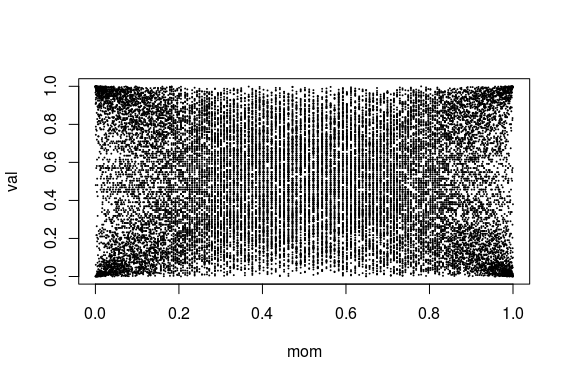
\includegraphics[scale=1]{obs}
\caption{Pseudo-Observations of the returns plotted against each other}
\end{figure}
\begin{figure}
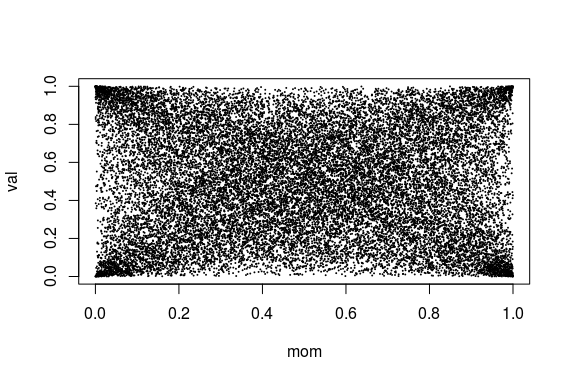
\includegraphics[scale=1]{res}
\caption{Pseudo-Observations of the residuals plotted against each other}
\end{figure}
\begin{figure}
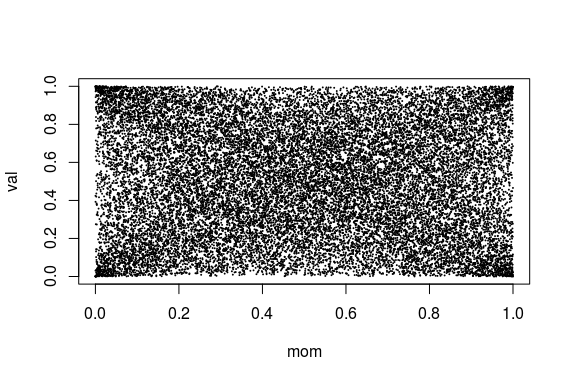
\includegraphics[scale=1]{stres}
\caption{Pseudo-Observations of the standardized residuals plotted against each other}
\end{figure}
\end{document}